% Doc class required by class assignment.
\documentclass{sig-alternate-05-2015}
\usepackage{graphicx}
\graphicspath{ {sections/architecture/i/}, {sections/progress/i/}  }
% copyright and other misc things provided by template.
% DOI
\doi{10.475/123_4}

% ISBN
\isbn{123-4567-24-567/08/06}

% Conference
\conferenceinfo{PLDI '13}{June 16--19, 2013, Seattle, WA, USA}

\acmPrice{\$15.00}
% end copyright
\begin{document}

% Paper title
\title{WolfTutor
  % \titlenote{(Paper 1). For use with
  % SIG-ALTERNATE.CLS. Supported by ACM.}
}
\subtitle{A system to enable peer tutoring built on Slack
  % \titlenote{A full version of this paper is available as
  % \textit{Author's Guide to Preparing ACM SIG Proceedings Using
  % \LaTeX$2_\epsilon$\ and BibTeX} at
  % \texttt{www.acm.org/eaddress.htm}
  % }
}

\numberofauthors{3} %  in this sample file, there are a *total*
\author{
  \alignauthor
  {Monica Metro}\\
  \affaddr{NC State University}\\
  %\affaddr{3021 F Dorner Circle}\\
  %\affaddr{Raleigh, NC}\\
  \email{mgmetro@ncsu.edu}
  % 2nd. author
  \alignauthor
  {Zachery DeLong}\\
  \affaddr{NC State University}\\
  %\affaddr{2305 Horizon Hike Ct}\\
  %\affaddr{Raleigh, NC}\\
  \email{zpdelong@ncsu.edu }
  % 3rd. author
  \alignauthor 
  {Zhangqi Zha} \\
  \affaddr{NC State University}\\
  %\affaddr{1800 Vienna Wood Dr}\\
  %\affaddr{Raleigh, NC}\\
  \email{zzha@ncsu.edu}
}
% Generate page header.
\maketitle

% Paper body
\begin{abstract}
In this abstract, we need to preview our experiment and our results 
\end{abstract}
%%% Local Variables:
%%% mode: latex
%%% TeX-master: "../main"
%%% End:


\section{Introduction}
\label{sec:intro}
What should an intro do?

\subsection{WolfTutor}
\label{sec:wolftutor}

In this section, we need to briefly explain what Wolftutor is

\subsection{Tutor Matching}
\label{sec:tutor-matching}

In this section, we should make the case that Wolftutor's matching needs
improvement and point out who would benefit from better matching/why.

This section should also introduce our system and explain why what we're doing
is appropriate.
%%% Local Variables:
%%% mode: latex
%%% TeX-master: "../main"
%%% End:


\section{Design}
\label{sec:design}
\subsection{Enhancement}
\label{sec:enhancement}
As mentioned in section \ref{sec:tutor-matching} the goal of this project is to
improve the matching done by WolfTutor.  In its original form, students input
only what subject they were interested in a tutor for and the system returned
back all students in that given subject.  While effective, this brute-force
strategy can wind up showing students an extremely large number of potential
tutors in their chat app, which can be somewhat challenging to navigate.

The original system also displayed fairly little information about the tutor
when searching.  The list of tutors returned by the ``find a tutor''
functionality contained basic information such as name and major, but did not
include information about the performance of the tutor academically or their
reviews.  To see reviews, the searching student would have to hit a ``review''
button which would then display all the reviews that tutor had at the bottom of
the screen. While this technically made the necessary information available,
this UI was challenging to use, and after getting feedback from the first round
of reviews, the team decided to make some changes to this process.  

First and foremost, however, the goal of this project is to improve the process
of chosing a tutor in WolfTutor by providing a filtered list of tutors to
students when they search for tutors in the system.  
%%% Local Variables:
%%% mode: latex
%%% TeX-master: "../main"
%%% End:


\subsection{Bugs}
\label{sec:bugs}
In this section we will talk about the issues we had to fix in the system before
working and how we helped avoid them in our new code

%%% Local Variables:
%%% mode: latex
%%% TeX-master: "../main"
%%% End:


\subsection{Use Cases}
\label{sec:use-cases}
testing
%%% Local Variables:
%%% mode: latex
%%% TeX-master: "../main"
%%% End:


\subsection{Architecture}
\label{sec:architecture}
\subsubsection{Overview}
\begin{figure*}[ht]
\label{arch-pic}
%\caption{Architecture Design}
\centering
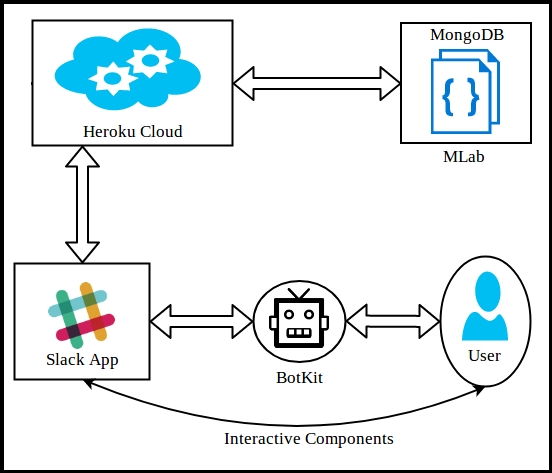
\includegraphics[height=0.5\textheight]{new_architecture.png}
\end{figure*}

Figure \ref{arch-pic} outlines the architecture of the application.
There are three main divisions: The user interface, the application server, and the database. 
Slack was used as the user interface. A custom bot was installed to that Slack page to handle 
interactive elements with the users. The applicaton was built with NodeJS. MongoDB was the 
database chosen to hold user data. For development purposes, a local server of NodeJS was run 
along with a local mongoDB database. Ngrok was used to tunnel webhooks between our local servers, 
which was necessary to get past local NATs and firewalls securely. The specific infrastructures are discussed as followed.


\subsubsection{Slack}
\label{sec:slack}

Slack is primarily a business tool intended to help facilitate
communication and coordination between individuals and groups at organizations.
In practice, however, Slack has become a familiar name with many unintended audiences such
as online communities and even university courses such as this one because of it's 
availability and ease of use. Attracting users to a platform they're already familiary with
is generally easier and less costly than attracting attention to a brand new website.

Another reason for using the Slack platform is that it already supports the languages and keyboard layouts for English, 
Japanese, German, Spanish, and French. Their website also claims to be 
including more regions in the future. Because of this, using a platform like Slack 
is beneficial to smaller developers as they can spend less time building a unique website 
and pushing it out internationally and more time on the functionality of the product. 

\paragraph{Slack Bot}
As mentioned previously, the target for this chat bot is to run in the Slack
platform. The Slack bot handles the interactions between the user and the NodeJS applications. 
All responses given by the user would be posted to the application by the bot. 
Similarily, all prompts sent to the user from application would be posted to Slack by the bot.

While it is true that this bot has been deployed to Slack specifically, it was
developed using a popular API called Botkit, which actually has APIs for
multiple chat services such as Facebook Messenger or Discord as well as Slack.
Because of this, it is possible to port WolfTutor to these other platforms
without needing to entirely start over.

%%% Local Variables:
%%% mode: latex
%%% TeX-master: "../main"
%%% End:


\subsubsection{NodeJS}
\label{sec:nodejs}
NodeJS is the primary framework being used in this project.  Node is a runtime
for Javascript which has proven to be strong competition for more traditional
LAMP stacks in the web.  In this case, it provides a number of different
libraries which make development of a chatbot easier.  Running Javascript also
has the benefit of making the chat bot easier to work on for a large number of
people given Javascripts ubiquity in recent years.

%%% Local Variables:
%%% mode: latex
%%% TeX-master: "../main"
%%% End:


\subsubsection{MongoDB}
\label{sec:mongo}
MongoDB has serveral advantages. It is well documented for use with NodeJS, it is easy to set up a local database, it is also easy to set up online with MLAB platform and integrate into Heroku, and it is also easy to access through authorization credentials. Creating and uploading a mock database with a python script only took seconds with MLAB's authorization abilities to allow us to access the database outside of the MLAB site portal.


%%% Local Variables:
%%% mode: latex
%%% TeX-master: "../main"
%%% End:


\subsubsection{Heroku}
\label{sec:heroku}
Heroku is a popular cloud platform service that enables 
developers to run their applications online. Because of its 
popularity, there is an ample amount of documentation for using Heroku among other services such as NodeJS and mongoDB. Heroku also offers a free personal server that was used to speed up
in person evaluations of WolfTutor. To start the server, the single free dyno of the application's server would execute the Procfile via the 'npm start' command.


%%% Local Variables:
%%% mode: latex
%%% TeX-master: "../main"
%%% End:







%%% Local Variables:
%%% mode: latex
%%% TeX-master: "../main"
%%% End:


\subsection{Infastructure}
\label{sec:infastructure}
testing
%%% Local Variables:
%%% mode: latex
%%% TeX-master: "../main"
%%% End:

\subsubsection{Slack}
\label{sec:slack}

Slack is primarily a business tool intended to help facilitate
communication and coordination between individuals and groups at organizations.
In practice, however, Slack has become a familiar name with many unintended audiences such
as online communities and even university courses such as this one because of it's 
availability and ease of use. Attracting users to a platform they're already familiary with
is generally easier and less costly than attracting attention to a brand new website.

Another reason for using the Slack platform is that it already supports the languages and keyboard layouts for English, 
Japanese, German, Spanish, and French. Their website also claims to be 
including more regions in the future. Because of this, using a platform like Slack 
is beneficial to smaller developers as they can spend less time building a unique website 
and pushing it out internationally and more time on the functionality of the product. 

\paragraph{Slack Bot}
As mentioned previously, the target for this chat bot is to run in the Slack
platform. The Slack bot handles the interactions between the user and the NodeJS applications. 
All responses given by the user would be posted to the application by the bot. 
Similarily, all prompts sent to the user from application would be posted to Slack by the bot.

While it is true that this bot has been deployed to Slack specifically, it was
developed using a popular API called Botkit, which actually has APIs for
multiple chat services such as Facebook Messenger or Discord as well as Slack.
Because of this, it is possible to port WolfTutor to these other platforms
without needing to entirely start over.

%%% Local Variables:
%%% mode: latex
%%% TeX-master: "../main"
%%% End:


\subsubsection{NodeJS}
\label{sec:nodejs}
NodeJS is the primary framework being used in this project.  Node is a runtime
for Javascript which has proven to be strong competition for more traditional
LAMP stacks in the web.  In this case, it provides a number of different
libraries which make development of a chatbot easier.  Running Javascript also
has the benefit of making the chat bot easier to work on for a large number of
people given Javascripts ubiquity in recent years.

%%% Local Variables:
%%% mode: latex
%%% TeX-master: "../main"
%%% End:


\subsubsection{Heroku}
\label{sec:heroku}
% TODO:




%%% Local Variables:
%%% mode: latex
%%% TeX-master: "../main"
%%% End:


\section{Evaluation}
\label{sec:evaluation}

\section{Conclusion}
\label{sec:conclusion}

\subsection{Results}
\label{sec:results}

\subsection{Future Work}
\label{sec:future-work}
\subsubsection{Further Evaluation}
\label{sec:further-evaluation}
The team has made a best effort to evaluate the algorithm presented in this
paper both using a manually-labeled data set and using in-person interviews with
potential users. That said, true evaluation of educational software must be done
in a classroom setting.  
% TODO: describe ideal study

\subsubsection{Future Enhancement}
% TODO: describe the process of implementing a new algorithm in this setting
\label{sec:future-enhancement}

%%% Local Variables:
%%% mode: latex
%%% TeX-master: "../main"
%%% End:


\subsection{Final Thoughts}
\label{sec:final-thoughts}
The final thought to conisder is whether or not group-p's contribution to
WolfTutor is truly an improvement over the existing system.
%%% Local Variables:
%%% mode: latex
%%% TeX-master: "../main"
%%% End:


%%% Local Variables:
%%% mode: latex
%%% TeX-master: "../main"
%%% End:




% REMOVE NOCITE OR IT WILL LIST EVERYTHING IN YOUR DATABASE AS A REFERENCE
% \nocite{*}

% Bibliography/style
\bibliographystyle{abbrv}

\bibliography{biblio}
% End bibliography/style

\end{document}
